%% ============================================================================
%%  When Chats Split Apart: Formalizing Temporal Communication Fragmentation
%%  and the CARTA Reconstruction Framework
%%
%%  Source of truth for prose: docs/DRAFT_PAPER.md
%%  Source of truth for notation/outline: docs/PAPER_BLUEPRINT.md
%%
%%  Build:  pdflatex main -> bibtex main -> pdflatex main -> pdflatex main
%%
%%  NOTE ON DOCUMENT CLASS: no venue beyond arXiv has been chosen, and the
%%  arXiv category itself is still open (docs/PAPER_BLUEPRINT.md line 4 lists
%%  cs.DL / cs.SE / cs.DC, unresolved). This uses a plain `article` class on
%%  purpose. Do NOT swap in IEEEtran/acmart until a venue is actually decided.
%% ============================================================================
\documentclass[11pt,a4paper]{article}

%% inputenc/fontenc are what pdflatex needs and what a Unicode engine
%% (xelatex, lualatex, tectonic) warns about. Guarding on the engine keeps the
%% build warning-free either way; the documented build is still pdflatex.
\usepackage{iftex}
\ifPDFTeX
  \usepackage[T1]{fontenc}
  \usepackage[utf8]{inputenc}
\fi
\usepackage[margin=1in]{geometry}

\usepackage{amsmath}
\usepackage{amssymb}
\usepackage{amsthm}

\usepackage{booktabs}
\usepackage{tabularx}
\usepackage{array}

\usepackage{algorithm}
\usepackage{algpseudocode}

%% Figures 1 and 2 are drawn in TikZ rather than shipped as image files, so the
%% paper source stays self-contained and the diagrams stay editable alongside
%% the prose they illustrate. No external image is used anywhere.
\usepackage{tikz}
\usetikzlibrary{arrows.meta,positioning,calc,fit,backgrounds,patterns,
                decorations.pathreplacing}

\usepackage{natbib}
\bibliographystyle{plainnat}

%% British spelling is deliberate in running prose (see docs/DRAFT_PAPER.md
%% drafting note 9). No spell-checking or hyphenation package may be added
%% that would Americanise it. `babel` with `british` is loaded for correct
%% hyphenation ONLY -- it does not alter spelling.
\usepackage[british]{babel}

%% Long code identifiers (e.g. AMBIGUOUS_DATE_FORMAT, owner/repo-name) cannot
%% be hyphenated without inserting a character that is not part of the
%% identifier, which would mislead in a paper whose subject is exact record
%% fidelity. emergencystretch relaxes interword spacing instead and inserts
%% nothing. Do not replace this with a \texttt hyphenation package.
\setlength{\emergencystretch}{3em}

\usepackage[hidelinks]{hyperref}
\usepackage{url}

%% The archived-snapshot URL in the WhatsApp reference is long enough that it
%% cannot break at default settings, which leaves a badness-10000 line in the
%% bibliography. This lets TeX break inside a URL without inserting any
%% character into it -- the same rule applied to code identifiers above.
\Urlmuskip=0mu plus 1mu\relax

%% ---------------------------------------------------------------------------
%%  UNRESOLVED CITATION MARKER -- currently UNUSED, kept on purpose.
%%
%%  \citeTODO renders a loud inline marker AND emits a LaTeX warning at every
%%  build, so an unresolved citation cannot survive a final read-through
%%  unnoticed. Its one use, [CITE-T2] in Section 1, was resolved on 2026-08-25
%%  and the call removed; the mechanism earned its keep by catching a claim
%%  that outran its source (docs/DRAFT_PAPER.md drafting note 1).
%%
%%  Kept so the next unsourced claim has somewhere to go. Use it rather than
%%  letting a placeholder citation compile quietly.
%% ---------------------------------------------------------------------------
\newcommand{\citeTODO}[1]{%
  \GenericWarning{}{%
    LaTeX Warning: UNRESOLVED CITATION -- #1 -- must be resolved before submission%
  }%
  \textbf{[\,UNRESOLVED CITATION: #1\,]}%
}

%% Shorthand for the CARTA reconstruction algebra, so the notation cannot
%% drift between sections.
\newcommand{\carta}{\ensuremath{%
  \mathcal{F} \rightarrow \mathcal{R} \rightarrow (\mathcal{R}', \mathcal{Q})
  \rightarrow (\mathcal{U}, \Omega)}}

%% NB: the line break below is \\ (two backslashes). A single trailing
%% backslash is a control space, not a break -- it compiles without error and
%% silently runs the title onto one line.
\title{When Chats Split Apart: Formalizing Temporal Communication\\
Fragmentation and the CARTA Reconstruction Framework}

\author{%
  Maitreya Sapariya\\
  Independent Researcher\\
  \href{https://orcid.org/0009-0003-9346-3775}{ORCID: 0009-0003-9346-3775}%
}
\date{\today}

\begin{document}
\maketitle

%% Abstract written 2026-08-25, after Sections 1--9 were final, from those
%% sections. Every claim in it is one the body already makes and sources:
%% the three conditions are Section 2.2, the contract and Q/Omega are
%% Sections 3.1/3.3/3.5, the "claim priority over none of them" sentence is
%% Section 8's opening argument, and the deferred-implementation scope is
%% Sections 5 and 6. It states no result, because the paper reports none.
\begin{abstract}
A single messaging account's history can end up split across two archives that
are each internally complete and that the platform will not recombine. We
characterise this state as Temporal Communication Fragmentation and give three
necessary conditions for it: a timeline that bifurcates when the primary device
becomes unavailable, both branches persisting and accumulating with no
synchronisation between them, and no platform operation yielding their union.
Nothing is destroyed. Both archives stay intact; what is missing is any
operation presenting them as one history. A restore that replaces rather than
merges leaves an intact archive unreachable through the platform holding it.

We then specify CARTA, a platform-agnostic three-stage reconstruction contract,
\carta. Records that cannot be interpreted unambiguously are routed to a
quarantine set $\mathcal{Q}$ under typed reason codes instead of being resolved
by guessing, and every reconstruction emits a report $\Omega$ carrying
provenance, quarantine carryover, conflicts and counts.

Merging chat archives is not new, and neither is staging forensic
reconstruction nor per-record provenance; we claim priority over none of them.
$\mathcal{Q}$ and $\Omega$ are what the tools and literature surveyed here do
not supply. This is a specification paper: the reference implementation is
deferred, and no evaluation is reported.
\end{abstract}

%% Section 1 -- Introduction & Motivation
%% Ported from docs/DRAFT_PAPER.md Section 1. British spelling is deliberate.

\section{Introduction \& Motivation}
\label{sec:introduction}

A phone stops working and goes in for repair. Its owner keeps the messaging
account running on a spare handset, and the conversations continue there for as
long as the repair takes. The original phone comes back. The owner restores the
most recent backup onto it, and the messages from the repair window vanish from
the screen.

Nothing was deleted. Those messages still sit in the spare device's local
database, and in any export the user thought to take before handing the account
back. The platform simply offers no operation that puts the two histories
together. WhatsApp's own restore guidance requires the same account that created
the backup~\citep{whatsapp_backup_restore}; it documents no operation for
combining two backups, a gap that has motivated the third-party merge tools
surveyed in Section~\ref{sec:related:tooling}.

We call this state \textbf{Temporal Communication Fragmentation} (TCF). Its
signature is a fully intact archive that the platform will not surface. The data
survives; the affordance to reach it does not.

Three properties make the situation harder than it first appears. The two
archives overlap in part and diverge in part, so neither is a superset of the
other. They carry no shared version history, no operation log, and no common
ancestor, because consumer chat exports were never designed to be reconciled.
And the restore operation that finalises the split gives no warning that a
competing archive exists, attempts no comparison, and reports nothing about what
it replaced.

\paragraph{Motivation, stated as motivation.}
This work began with one of the authors losing a stretch of message history to
exactly this sequence: primary handset unavailable, account carried on a second
handset, history replaced on restore. That incident prompted the research
questions below. It is an anecdote. It is not evidence, no controlled experiment
was run against it, and no claim in this paper rests on it.

The paper asks three questions:

\begin{description}
  \item[RQ1.] What conditions must hold for a single account's message history to
    end up split across two archives that are each internally complete and
    mutually irreconcilable through the platform?
  \item[RQ2.] Given two or more such archives, what does a reconstruction
    procedure have to guarantee for its output to be trustworthy as a record,
    rather than merely plausible?
  \item[RQ3.] Where do those guarantees sit relative to what optimistic
    replication, digital forensics, and the existing body of chat-merging tools
    already provide?
\end{description}

Answering RQ1 gives a formal characterisation of TCF with three necessary
conditions (Section~\ref{sec:tcf}). Answering RQ2 gives CARTA (Chat Archive
Reconstruction \& Temporal Access), a platform-agnostic specification of a
three-stage reconstruction contract, \carta, in which the data passed between
stages is typed, records that cannot be safely interpreted are retained in a
quarantine set $\mathcal{Q}$ rather than dropped, and every reconstruction emits
a structured report $\Omega$ covering provenance, quarantine carryover,
conflicts, and counts (Sections~\ref{sec:carta} and~\ref{sec:algorithms}).
Answering RQ3 is Section~\ref{sec:related}.

\paragraph{What this paper does not do.}
No implementation is evaluated here. CHAMP-Pipeline, the WhatsApp-specific
reference implementation of CARTA, is described in
Section~\ref{sec:implementation} as planned work and does not yet exist;
\texttt{core/src/\{ingestion,normalization,synthesis\}/} are empty. There is
accordingly no benchmark, no performance measurement, and no
reconstruction-accuracy figure anywhere in this paper. Where a capability is
stated, it is either a property the specification requires of a conforming
implementation or a citation to someone else's system. Readers should treat the
contribution as a problem definition and a specification, with implementation
and evaluation left as declared future work.

%% Section 2 -- Temporal Communication Fragmentation
%% Ported from docs/DRAFT_PAPER.md Section 2. British spelling is deliberate.

\section{Temporal Communication Fragmentation}
\label{sec:tcf}

\subsection{Definition}
\label{sec:tcf:definition}

\textbf{Temporal Communication Fragmentation} is a state in which a user's
communication history for a single logical account becomes fragmented across
two or more device-bound application instances that persist independently, and
for which the platform provides no operation yielding their union. It arises
from primary-device unavailability, continued account use on a secondary
device during that window, and primary-device recovery.

The definition requires the absence of a union-yielding operation and nothing
further. How a given platform declines to provide one is a separate, empirical
matter. On the platform examined here, every path that brings the archives back
together, restore above all, substitutes one state for another rather than
merging them, with no user-facing warning that a competing archive exists and
no attempt at a diff or a reconciliation. That is an observation about one
documented restore path, not a property TCF requires.

We assert the observable restore behaviour and nothing about the backend that
produces it. A single-slot, last-write-wins cloud backup destination would
explain what users see, but we have found no vendor documentation, citation, or
controlled experiment establishing that architecture, and no argument in this
paper depends on it.

%% Figure 1 -- TCF timeline. Drawn from Section 2.2 only: the three necessary
%% conditions, the t_f / t_r landmarks, and the F_1 / F_2 extents with delta
%% and epsilon. Nothing here is asserted that Section 2.2 does not already
%% state. delta and epsilon are drawn strictly positive because that is the
%% case the prose singles out as the reason deduplication is needed at all
%% (Sections 2.2 and 3.4); both are defined as merely non-negative, and the
%% caption says so rather than letting the drawing imply otherwise.
%%
%% NB (2026-08-26, ground-problem alignment): C1 and C2 are events and sit on
%% the timeline; C3 is a standing property of the platform and must NOT be
%% drawn at a point. It spans from t_f onwards. The restore is drawn dashed
%% and labelled as the manifest case only -- conditions 1-3 are already
%% satisfied without it. Reverting either of those would reintroduce the
%% overfitting this pass removed.
\begin{figure}[htbp]
  \centering
  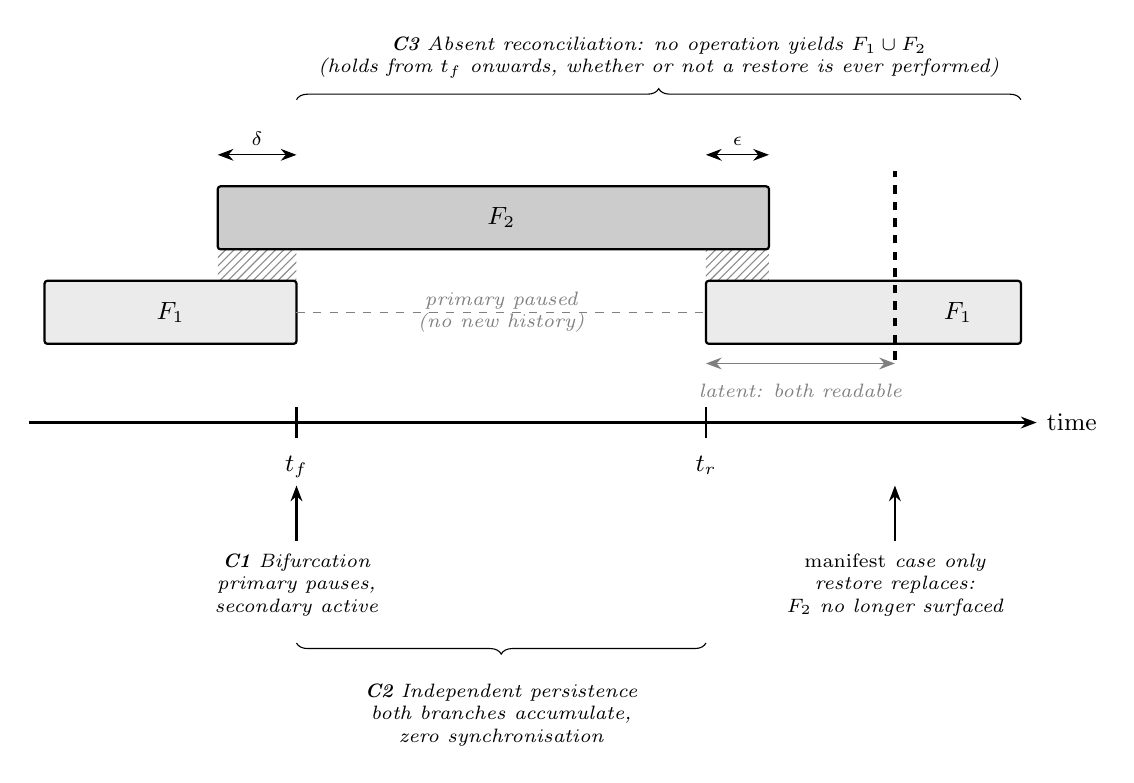
\begin{tikzpicture}[
      x=1mm, y=1mm,
      >={Stealth[length=2mm]},
      frag/.style={rounded corners=1pt, draw, thick},
      lbl/.style={font=\small},
      tick/.style={draw, thick},
      cond/.style={font=\scriptsize\itshape, align=center},
    ]

    %% landmark positions
    \def\tf{34}   % device failure / bifurcation
    \def\tr{86}   % primary device recovery
    \def\trest{110} % restore, if it is ever performed
    \def\dlt{10}  % delta : pre-existing history on the secondary
    \def\eps{8}   % epsilon: lag before the account returns to the primary

    %% ---- C3 : a standing property, not an event -------------------------
    \draw[decorate, decoration={brace, amplitude=4pt}] (\tf,41) -- (126,41);
    \node[cond, above=1.5mm] at ({(\tf+126)/2},41)
      {\textbf{C3} Absent reconciliation: no operation yields
       $F_1 \cup F_2$\\(holds from $t_f$ onwards, whether or not
       a restore is ever performed)};

    %% ---- time axis -------------------------------------------------------
    \draw[->, thick] (0,0) -- (128,0) node[right, lbl] {time};

    \foreach \x in {\tf, \tr} {
      \draw[tick] (\x,-2) -- (\x,2);
    }
    \node[lbl, below=1mm] at (\tf,-2) {$t_f$};
    \node[lbl, below=1mm] at (\tr,-2) {$t_r$};

    %% ---- F_1 : primary -- paused across the window ------------------------
    \draw[frag, fill=black!8] (2,10) rectangle (\tf,18);
    \draw[frag, fill=black!8] (\tr,10) rectangle (126,18);
    \draw[dashed, gray] (\tf,14) -- (\tr,14);
    \node[lbl] at (18,14) {$F_1$};
    \node[lbl] at (118,14) {$F_1$};
    \node[cond, gray] at ({(\tf+\tr)/2},14) {primary paused\\(no new history)};

    %% ---- F_2 : secondary -- active across the window ----------------------
    \draw[frag, fill=black!20] ({\tf-\dlt},22) rectangle ({\tr+\eps},30);
    \node[lbl] at ({(\tf+\tr)/2},26) {$F_2$};

    %% ---- the two overlap regions -----------------------------------------
    \begin{scope}[on background layer]
      \fill[pattern=north east lines, pattern color=black!45]
        ({\tf-\dlt},10) rectangle (\tf,30);
      \fill[pattern=north east lines, pattern color=black!45]
        (\tr,10) rectangle ({\tr+\eps},30);
    \end{scope}
    \draw[<->] ({\tf-\dlt},34) -- (\tf,34)
      node[midway, above, font=\scriptsize] {$\delta$};
    \draw[<->] (\tr,34) -- ({\tr+\eps},34)
      node[midway, above, font=\scriptsize] {$\epsilon$};

    %% ---- latent TCF : C1-C3 hold, both archives still readable -----------
    %% Single line, anchored inside the 0--10 gap. Do not re-anchor this above
    %% its arrow: it then rides up into the right-hand F_1 rectangle.
    \draw[<->, gray] (\tr,7.5) -- (\trest,7.5);
    \node[cond, gray] at ({(\tr+\trest)/2},4)
      {latent: both readable};

    %% ---- the restore, if performed : latent becomes manifest -------------
    \draw[very thick, dashed] (\trest,8) -- (\trest,32);

    %% ---- below-axis annotations, in three non-overlapping bands ----------
    %% band 1 (y -8 to -26): C1 at t_f and the manifest note at the restore;
    %% they do not overlap horizontally. Arrows start at -8, below the tick
    %% labels, so they do not strike through $t_f$ / $t_r$.
    \draw[->, thick] (\tf,-15) -- (\tf,-8);
    \node[cond, below=0.5mm] at (\tf,-15)
      {\textbf{C1} Bifurcation\\primary pauses,\\secondary active};

    \draw[->, thick] (\trest,-15) -- (\trest,-8);
    \node[cond, below=0.5mm] at (\trest,-15)
      {\emph{manifest} case only\\restore replaces:\\$F_2$ no longer surfaced};

    %% band 2 (y -28 down): C2, spanning t_f to t_r, clear of band 1.
    \draw[decorate, decoration={brace, amplitude=4pt, mirror}]
      (\tf,-28) -- (\tr,-28);
    \node[cond, below=2mm] at ({(\tf+\tr)/2},-30)
      {\textbf{C2} Independent persistence\\both branches accumulate,\\zero synchronisation};

  \end{tikzpicture}
  %% Caption describes what is drawn. The argument behind the drawing --- why
  %% C3 is a span rather than a point, why the restore is optional, why the
  %% overlap needs deduplication --- is in Section 2.2 and must not migrate
  %% back up here (peer review, Minor 13: a caption doing expository work).
  \caption{Temporal Communication Fragmentation on a timeline, with the three
  necessary conditions of Section~\ref{sec:tcf:conditions} marked. $F_1$ holds
  messages with $t(m) \le t_f$ or $t(m) \ge t_r$; $F_2$ holds messages in
  $[t_f - \delta,\, t_r + \epsilon]$. Hatching marks the two overlap regions.
  $\delta$ and $\epsilon$ are non-negative in the model and are drawn here as
  strictly positive so that the overlap is visible. C1 and C2 are drawn as
  points and C3 as a span; the restore is dashed because it is optional.}
  \label{fig:tcf_timeline}
\end{figure}

\subsection{Necessary conditions}
\label{sec:tcf:conditions}

TCF requires all three of the following to hold at once
(Figure~\ref{fig:tcf_timeline}).

\paragraph{Condition 1, Bifurcation.}
At failure time $t_f$, one authoritative timeline splits into two independently
updating branches. The primary is paused; the secondary is active.

\paragraph{Condition 2, Independent persistence.}
Both branches survive and accumulate new history for some duration with zero
synchronisation between them. This condition does most of the work in separating
TCF from the replication literature, and Section~\ref{sec:related:replication}
returns to it.

\paragraph{Condition 3, Absent reconciliation.} No platform-native
operation yields the union of the two archives. This condition is a property of
the platform's reunification semantics rather than an event that must occur. It
holds from the moment the branches exist, whether or not the user ever invokes
one of those paths, and it is what separates TCF from the
optimistic-replication systems of Section~\ref{sec:related:replication}, which
attempt reconciliation imperfectly rather than declining to attempt it.

Whether a platform's substitutive paths also overwrite silently, warn, or offer
a comparison bears on how much a user can recover unaided, not on whether the
condition holds. In the restore path examined here none of those mitigations is
present: restoration overwrites current chat state instead of merging into it,
surfaces no warning, and gives no indication that a second archive existed.
That is the observed behaviour of one platform, recorded because it is the
motivating case, and Condition 3 does not depend on it.

Stated most carefully, Condition 3 is a property of the reconstruction problem's
input rather than a claim about any company's feature list: the fragments carry
no shared reconciliation state, and no union-yielding operation is available to
the user holding them. This matters for what a changelog can do to this paper. If
a platform ships a merge affordance tomorrow, instances of TCF on that platform
cease to arise, in the same way that a fix removes instances of a defect class
without refuting its description. What the definition would lose is reach, not
correctness --- and the reconstruction problem for archives already fragmented
before such a fix would be untouched, because the fragments in hand would still
carry no shared reconciliation state. A definition whose truth conditions sat
inside a vendor's roadmap would be a poor research object; this one names a
configuration that either obtains for a given pair of archives or does not.

\paragraph{Latent and manifest fragmentation.} Conditions 1 to 3 are satisfied
while both archives remain individually readable on their own devices; what is
unavailable is any view spanning them. We call this the \emph{latent} case,
and it is the case the motivating incident of Section~\ref{sec:introduction}
exhibits. A restore makes the fragmentation \emph{manifest}: the replaced
archive thereafter survives only in whatever unsynced local form remains on
the device holding it, and the platform ceases to surface it at all. Manifest
fragmentation is the severe case of TCF, not its definition. The distinction
matters for how urgent reconstruction is and for what a user can still recover
unaided, but not for the reconstruction problem itself, because both cases
present the same input: independently preserved fragments carrying no shared
reconciliation state.

Formally (Section~\ref{sec:carta} develops this), device failure at $t_f$ and
recovery at $t_r$ split a ground-truth history $\mathcal{T}$ into $F_1$,
holding messages with $t(m) \le t_f$ or $t(m) \ge t_r$, and $F_2$, holding
messages in $[t_f - \delta,\, t_r + \epsilon]$. The parameters $\delta$ and
$\epsilon$ are non-negative, representing pre-existing history on the
secondary device and the lag before the account returns to the primary. Both
may be strictly positive, so $F_1$ and $F_2$ can overlap. That overlap is why
reconstruction needs deduplication rather than concatenation.

%% Added 2026-08-26 after review: the motivating incident is the delta = 0
%% boundary, and the paper previously asserted overlap as though it were
%% general without saying where the general case comes from. Do not delete
%% without also softening Section 1's "overlap in part" and Section 3.4's
%% "deduplication exists because of this overlap".
The boundary case $\delta = \epsilon = 0$ deserves explicit mention, because it
is the one the motivating incident of Section~\ref{sec:introduction} exhibits:
the secondary device was set up without restoring any prior history, so $F_2$
begins empty at $t_f$ and $F_1 \cap F_2 = \emptyset$. Reconstruction there
reduces to ordered concatenation, and none of the deduplication machinery of
Section~\ref{sec:algorithms} is exercised. We do not treat that case as the
general one. A secondary device is more often brought into service the way any
replacement device is, by restoring whatever backup exists, and a backup made
before $t_f$ carries pre-failure history that the primary also still holds ---
which is exactly $\delta > 0$. Symmetrically, an account does not always return
to the primary the moment it is repaired, and any use of the secondary after
$t_r$ produces $\epsilon > 0$. The overlapping configuration is therefore the
one a specification has to be written for, and the disjoint one is the easy
special case that falls out of it. Assuming disjointness and discovering
overlap later would mean a reconstruction that silently reported the overlap
region twice.

Where this paper calls a fragment \emph{internally complete}, it means
well-formed and gap-free with respect to its own accumulation window, which is
a property of each fragment considered separately. It is not a claim that
either fragment covers $\mathcal{T}$; by construction neither does, and that
is the whole difficulty. Internal completeness is an idealisation of the TCF
model rather than a property established of any real archive, and
Section~\ref{sec:discussion:incomplete} treats the case where it fails.

\subsection{Distinction from backup staleness}
\label{sec:tcf:staleness}

Backup staleness is the documented problem of infrequent snapshots losing data
when a device fails. One timeline exists, and the data from the unprotected
window was never captured. TCF has two timelines, each holding messages the other
lacks, both physically present. The reconstruction problem is one of retrieval
and reconciliation rather than of recovery from destruction.

\subsection{Position against neighbouring phenomena}
\label{sec:tcf:neighbours}

%% Table 1 -- Taxonomy of neighbouring data-loss and consistency phenomena.
%% Reproduced unchanged from docs/DRAFT_PAPER.md Section 2.4, which in turn
%% reproduces docs/PAPER_BLUEPRINT.md Section 4. \input from 02_tcf.tex.
%%
%% Note: the column headings and the TCF column use the source documents'
%% spelling ("Platform Behavior") rather than being Anglicised, because the
%% table is reproduced verbatim. See docs/DRAFT_PAPER.md drafting note 5.

\begin{table}[htbp]
  \centering
  \caption{Taxonomy of neighbouring data-loss and consistency phenomena.}
  \label{tab:taxonomy}
  \small
  \setlength{\tabcolsep}{4pt}
  \renewcommand{\arraystretch}{1.25}
  \begin{tabularx}{\textwidth}{@{}l >{\raggedright\arraybackslash}X >{\raggedright\arraybackslash}X >{\raggedright\arraybackslash}X >{\raggedright\arraybackslash}X@{}}
    \toprule
    \textbf{Dimension} &
      \textbf{Backup Staleness} &
      \textbf{Sync Conflict} &
      \textbf{Git 3-Way Merge} &
      \textbf{TCF (This Paper)} \\
    \midrule
    \textbf{Underlying Cause} &
      Infrequent snapshotting &
      Concurrent multi-client writes &
      Divergent commit histories &
      Device switch + independent persistence; no merge operation \\

    \textbf{Number of Timelines} &
      Exactly 1 &
      2+ concurrent &
      2 branches + Common Ancestor &
      2 independently persistent, potentially overlapping \\

    \textbf{Platform Behavior} &
      Restores stale snapshot &
      Rejection or branch fork &
      Automatic merge or conflict markers &
      \textbf{No operation yields the union; every reunification path replaces} \\

    \textbf{Physical Data State} &
      Missing (never recorded) &
      Present on server &
      Merged in working tree &
      \textbf{Intact on both devices; no combined view} \\

    \textbf{Resolution Target} &
      Data unrecoverable from the snapshot &
      Operational state restored &
      Codebase reconciliation &
      \textbf{Forensic reconstruction ($\mathcal{U}, \Omega$)} \\
    \bottomrule
  \end{tabularx}
\end{table}


Two further neighbours deserve separate treatment because they are close enough
to invite misreading, and both are already-named phenomena rather than gaps.

\paragraph{Sync conflict.}
Systems built for optimistic replication also allow replicas to diverge, and they
define conflict as a first-class condition. \citet{saito2005optimistic} survey
the area and describe divergence and conflict as the characteristic problems such
systems face. The difference is what happens on reunification: those platforms
attempt reconciliation, imperfectly and with human fallback, whereas the platform
behaviour in Condition 3 makes no attempt at all.

\paragraph{Device migration.}
Moving an account between handsets is routine, and the HCI literature on
multi-device use describes the resulting failure as information stranded on the
device the user is not currently holding~\citep{dearman2008othercomputer}.
Migration moves one continuous timeline. TCF requires two timelines that
accumulated independently and concurrently.

\subsection{Terminology: what TCF is not called}
\label{sec:tcf:terminology}

Three established terms sit close enough to ``temporal communication
fragmentation'' that a reader may reasonably assume the phenomenon is already
covered. Each denotes something else, and we set the boundaries explicitly rather
than rely on context.

\paragraph{Information fragmentation (personal information management).}
\citet{karger2006unification} define this as personal information split by the
very tools meant to manage it, with applications storing data ``in their own
particular locations and representations, inaccessible to other applications'';
the project-level variant is treated by Bergman and
colleagues~\citep{bergman2006project}. Later usage in the field routinely extends
the term across devices as well as applications, so the surface overlap with TCF
is real. Two things separate them. The unit differs: information fragmentation
concerns \emph{different items} bearing on one task or project, scattered across
stores, whereas TCF concerns \emph{one item stream}, a single conversation, split
into disjoint temporal segments. And the access status differs: fragmented
personal information is scattered but reachable, and the research goal is
unification across silos, whereas in TCF one intact archive is unreachable
through the platform that holds it. Karger and Jones do treat duplicate copies
drifting out of step, which is content divergence between copies a user made;
TCF's divergence is temporal, between copies the platform made and then rendered
mutually exclusive.

\paragraph{Fragmented communication (CSCW and workplace studies).}
In that literature the term describes one conversation spread across many
channels and tools. TCF is the opposite arrangement: one channel, one account,
one conversation, split by time rather than by venue.

\paragraph{Temporal fragmentation (time geography and ICT studies).}
\citet{hubers2008temporal} use this for the splitting of human \emph{activities}
into pieces performed at different times and places. The referent is an activity
pattern, not a data archive. We keep the name Temporal Communication
Fragmentation because the qualifier ``communication'' and the archival framing
distinguish the two, and because no prior work applies any of these three terms
to the configuration defined in Section~\ref{sec:tcf:conditions}. The collision
is nonetheless a live source of confusion, and it is the reason this subsection
exists.

%% Section 3 -- The CARTA Architectural Framework
%% Ported from docs/DRAFT_PAPER.md Section 3. Math ported verbatim from the
%% draft, which in turn follows docs/PAPER_BLUEPRINT.md 2.2-2.4 (locked).
%%
%% FOUR LOCKED CORRECTIONS -- do not regress any of these:
%%   1. F_1 / F_2 overlap is a feature (delta, epsilon >= 0), not disjointness.
%%   2. ~_dedup is a SIMILARITY relation feeding RECONCILIATION CLUSTERS. No
%%      "equivalence class" or quotient notation anywhere.
%%   3. Idempotence is a softened specification-level target, not a proven
%%      equation S(U,U) = (U, Omega).
%%   4. Normalization has THREE outcomes, not two.

\section{The CARTA Architectural Framework}
\label{sec:carta}

CARTA specifies how to get from a set of fragmented exports to one reconstructed
history together with an account of how that history was produced. It is a
specification and not a system: it fixes what each stage receives, what each
stage emits, and what the result must be able to report about its own
construction. Section~\ref{sec:implementation} describes the planned
implementation, and nothing in this section depends on that implementation
existing.

\subsection{The reconstruction algebra}
\label{sec:carta:algebra}

Write the raw fragment exports as $\mathcal{F} = \{F_1, F_2, \dots, F_n\}$. CARTA
composes three stages (Figure~\ref{fig:carta_pipeline}):

\begin{equation}
  \mathcal{F}
  \xrightarrow{\;\mathcal{I}\;} \mathcal{R}
  \xrightarrow{\;\mathcal{N}\;} (\mathcal{R}', \mathcal{Q})
  \xrightarrow{\;\mathcal{S}\;} (\mathcal{U}, \Omega)
  \label{eq:algebra}
\end{equation}

%% Figure 2 -- CARTA pipeline. The stage signatures are those of Sections 3.2
%% to 3.5, and the caption's contract is the \carta macro from main.tex, so
%% the diagram cannot drift from the text. Two structural facts the prose
%% makes explicit are drawn rather than described: Ingestion and Normalization
%% run per fragment with no cross-fragment reconciliation (3.2), and Synthesis
%% is the only stage that sees fragments together (3.4). The Q path is drawn
%% bypassing Synthesis into Omega, which is what 3.5's quarantine carryover
%% says: quarantined records are carried into the report, not reconciled.
\begin{figure}[htbp]
  \centering
  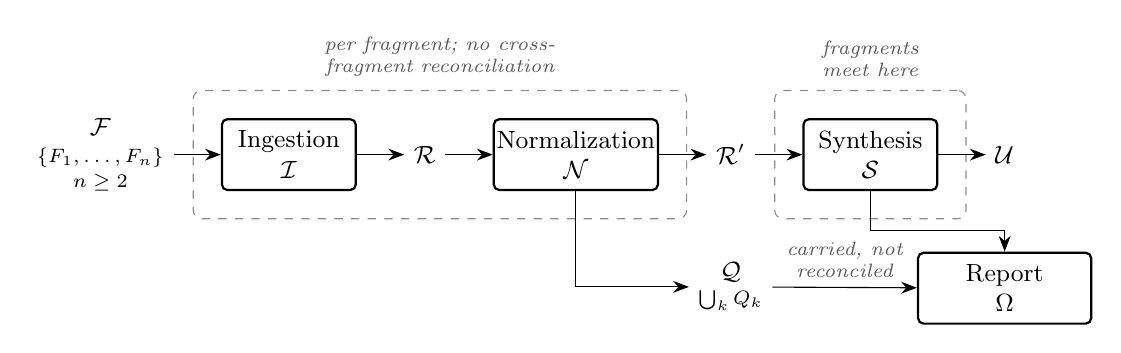
\begin{tikzpicture}[
      >={Stealth[length=2mm]},
      stage/.style={draw, thick, rounded corners=2pt, minimum height=9mm,
                    minimum width=17mm, align=center, font=\small,
                    inner xsep=1pt},
      data/.style={align=center, font=\small},
      note/.style={font=\scriptsize\itshape, align=center, text=black!65},
      node distance=9mm and 6mm,
    ]

    %% ---- per-fragment lane: Ingestion then Normalization ------------------
    \node[data] (F) {$\mathcal{F}$\\[-1pt]
      {\scriptsize$\{F_1,\dots,F_n\}$}\\[-2pt]
      {\scriptsize$n \ge 2$}};
    \node[stage, right=of F]        (I) {Ingestion\\$\mathcal{I}$};
    \node[data,  right=of I]        (R) {$\mathcal{R}$};
    \node[stage, right=of R]        (N) {Normalization\\$\mathcal{N}$};
    \node[data,  right=of N]        (Rp) {$\mathcal{R}'$};
    \node[stage, right=of Rp]       (S) {Synthesis\\$\mathcal{S}$};
    \node[data,  right=of S]        (U) {$\mathcal{U}$};

    \draw[->] (F) -- (I);
    \draw[->] (I) -- (R);
    \draw[->] (R) -- (N);
    \draw[->] (N) -- (Rp);
    \draw[->] (Rp) -- (S);
    \draw[->] (S) -- (U);

    %% ---- the quarantine path ---------------------------------------------
    \node[data, below=10mm of Rp] (Q) {$\mathcal{Q}$\\[-2pt]
      {\scriptsize$\bigcup_k Q_k$}};
    \draw[->] (N.south) |- (Q.west);

    \node[stage, below=10mm of U, minimum width=22mm] (Om)
      {Report\\$\Omega$};
    \draw[->] (Q) -- (Om)
      node[midway, above, note] {carried, not\\reconciled};
    \draw[->] (S.south) -- ++(0,-5mm) -| (Om.north);

    %% ---- scope annotations, both stated in the prose ---------------------
    \begin{scope}[on background layer]
      \node[draw, dashed, black!45, rounded corners=3pt,
            fit=(I)(N), inner sep=3.5mm] (perfrag) {};
      \node[draw, dashed, black!45, rounded corners=3pt,
            fit=(S), inner sep=3.5mm] (joint) {};
    \end{scope}
    \node[note, above=0.5mm of perfrag, text width=48mm]
      {per fragment; no cross-fragment reconciliation};
    \node[note, above=0.5mm of joint] {fragments\\meet here};

  \end{tikzpicture}
  \caption{The CARTA reconstruction contract \carta. Ingestion and
  Normalization operate on one fragment at a time and perform no
  reconciliation across fragments (Sections~\ref{sec:carta:ingestion}
  and~\ref{sec:carta:normalization}); Synthesis is the only stage that sees
  fragments together (Section~\ref{sec:carta:synthesis}). Records that fail to
  parse, and records that parse under more than one reading, both leave
  Normalization as $\mathcal{Q}$ and are carried into $\Omega$ with their
  reason codes rather than being resolved or discarded
  (Section~\ref{sec:carta:report}).}
  \label{fig:carta_pipeline}
\end{figure}

The quarantine set $\mathcal{Q}$ appears in the top-level algebra by design.
Records that cannot be interpreted safely are an output of the pipeline rather
than an internal concern of one stage, and writing them into the signature is
what makes it impossible for a conforming implementation to discard them quietly.

TCF as defined in Section~\ref{sec:tcf} is a two-way split: one primary device
pauses while one secondary continues, and Definition~1 formalises that case with
$n = 2$. CARTA's algebra is stated for $n \ge 2$. Nothing in the reconstruction
problem requires exactly two fragments, and a user who suffers repeated device
failures can accumulate more. The generalisation runs one way: CARTA covers more
than TCF's minimal case, while TCF itself remains binary.

\subsection{Ingestion}
\label{sec:carta:ingestion}

Ingestion maps each fragment independently to a sequence of structured records:

\begin{equation}
  \mathcal{I}: F_k \mapsto R_k
  = \langle r_{k,1}, r_{k,2}, \dots, r_{k,M_k} \rangle
\end{equation}

Each record keeps the raw text slice, the raw timestamp string, the raw sender
token, a message category, and a provenance tuple:

\begin{equation}
  \mathrm{prov}(r_{k,j}) = \big\langle
    \texttt{source\_id}: F_k,\;
    \texttt{line\_range}: [\ell_{\text{start}}, \ell_{\text{end}}],\;
    \texttt{sha256}: h(F_k)
  \big\rangle
  \label{eq:prov}
\end{equation}

Three parts, three jobs. The source identifier says which fragment the record
came from. The line range makes the original text re-locatable, so a reader can
return to the bytes the record was derived from. The hash binds that claim to a
specific file state, which is what allows an auditor to detect that the fragment
has changed since the reconstruction ran.

Ingestion is non-lossy and non-destructive. It writes nothing back to the
fragment files, and it filters no content. It also performs no reconciliation
across fragments, and this restriction is deliberate rather than incidental: a
stage that both parses and reconciles would make it impossible to say afterwards
whether a discrepancy came from a parsing decision or a merging decision.
Ingestion parses. Reconciliation happens later, once, in one place.

\subsection{Normalization}
\label{sec:carta:normalization}

Normalization converts each fragment's records into a shared canonical schema,
with UTC timestamps, resolved sender identity, and a fixed message-type taxonomy:

\begin{equation}
  \mathcal{N}: R_k \mapsto (R'_k, Q_k)
\end{equation}

Each record meets one of three fates, and the third is the one that distinguishes
this stage from a conventional parser.

A record that conforms to the canonical grammar \textbf{unambiguously} becomes a
canonical record in $R'_k$, carrying a UTC epoch timestamp, a normalised sender
identity, and a typed payload. Unambiguous here means a date and time admitting a
single valid interpretation, valid UTF-8, and a sender or system token that
resolves.

A record that \textbf{fails to parse} moves to the quarantine set $Q_k$.

A record that \textbf{parses but admits more than one reading} also moves to
$Q_k$. The date string \texttt{03/04/24} is the standard case: it is well-formed
under both day-month-year and month-day-year conventions, and nothing inside the
record itself decides between them. Such a record is not normalised, and it is
not resolved by picking the more likely convention. Guessing here would convert
an uncertainty into an assertion that later stages, and eventually the reader,
would have no way to distinguish from an observation.

Every quarantined record carries a typed reason code $\rho$. The taxonomy
distinguishes at minimum \texttt{MALFORMED\_\allowbreak TIMESTAMP},
\texttt{UNSUPPORTED\_\allowbreak FORMAT}, \texttt{AMBIGUOUS\_\allowbreak DATE\_\allowbreak FORMAT},
\texttt{UNRESOLVED\_\allowbreak SENDER}, and \texttt{INVALID\_\allowbreak ENCODING}, which separates a
record that could not be read from one that could be read in several ways. The
distinction matters downstream, because the two call for different remedies: a
malformed record may need a parser fix, whereas an ambiguous one may be resolvable
by evidence outside the record, such as a locale established elsewhere in the same
fragment.

Normalization is required to carry every record's provenance through to $R'_k$ or
$Q_k$. This is a guarantee the stage owes, and not a property Synthesis may assume
on its behalf.

\subsection{Synthesis}
\label{sec:carta:synthesis}

Synthesis is the only stage that sees fragments together:

\begin{equation}
  \mathcal{S}: \big(\{R'_1, \dots, R'_n\}, \{Q_1, \dots, Q_n\}\big)
  \mapsto (\mathcal{U}, \Omega)
\end{equation}

It performs four operations on the union
$\mathcal{R}'_{\text{all}} = \bigcup_{k=1}^{n} R'_k$, in this order: it orders the
records chronologically, groups records that appear to describe the same message
into reconciliation clusters, synthesises one canonical record per cluster, and
detects observations that cannot be reconciled. Section~\ref{sec:algorithms}
gives the procedure.

Recall from Section~\ref{sec:tcf:conditions} that $\delta$ and $\epsilon$ may both
be strictly positive, so $F_1$ and $F_2$ can overlap. A message sent during that
overlap appears in both fragments and arrives at Synthesis twice, in two
separately parsed forms that need not agree byte for byte. Deduplication exists
because of this overlap. Without it, concatenation would report the overlap region
twice and misrepresent the history it claims to reconstruct.

A conflict is any set of two or more observations that cannot be reconciled
deterministically under the reconstruction rules. This is broader than a timestamp
collision, and it includes contradictory sender attribution and orderings that
cannot both hold.

\subsection{The reconstruction report}
\label{sec:carta:report}

$\Omega$ is a first-class output with four components:

\begin{equation}
  \Omega = \big\langle
    \Omega_{\text{provenance}},\;
    \Omega_{\text{quarantine}} = \textstyle\bigcup_k Q_k,\;
    \Omega_{\text{conflicts}},\;
    \Omega_{\text{stats}}
  \big\rangle
  \label{eq:omega}
\end{equation}

The \textbf{provenance map} records, for every record in $\mathcal{U}$, its origin
device, origin export, origin backup date, and confidence. The \textbf{quarantine
carryover} holds every record from every $Q_k$, retained with its reason code
rather than dropped at the stage boundary. The \textbf{conflict log} holds every
irreconcilable observation under the definition above. The \textbf{statistics}
report deduplication counts along with resolved and unresolved ambiguity counts.

Quarantine carryover is the component that does the most work. A reconstruction
that silently omits what it could not handle looks identical, to its reader, to
one that had nothing to omit. Carrying $\mathcal{Q}$ into $\Omega$ makes the two
cases distinguishable without requiring the reader to re-run anything.

\subsection{Design principles}
\label{sec:carta:principles}

\paragraph{Deterministic.}
Identical fragment inputs produce an identical $(\mathcal{U}, \Omega)$.

\paragraph{Auditable.}
Every record in $\mathcal{U}$ traces back to at least one source fragment through
its provenance.

\paragraph{Non-destructive.}
Original fragment files are read and never modified.

\subsection{Invariants}
\label{sec:carta:invariants}

Four invariants constrain any conforming implementation.

\paragraph{Invariant 1, Zero unaccounted loss.}
Every ingested record either contributes provenance to a record in the unified
archive or appears in the quarantine carryover:

\begin{equation}
  \forall r \in \bigcup_{k=1}^{n} R_k, \quad
  \big(\exists u \in \mathcal{U} : \mathrm{prov}(r) \subseteq \mathrm{prov}(u)\big)
  \;\lor\;
  \big(\exists q \in \Omega_{\text{quarantine}} : q = r\big)
  \label{eq:inv1}
\end{equation}

No third outcome is permitted. A record cannot leave the pipeline unaccounted for.

\paragraph{Invariant 2, Strict provenance traceability.}
Every record in the unified archive carries at least one provenance entry, and
every entry references a valid source fragment:

\begin{equation}
  \forall u \in \mathcal{U}, \quad
  |\mathrm{prov}(u)| \ge 1
  \;\land\;
  \forall p \in \mathrm{prov}(u),\; p \text{ references a valid } F_k
  \label{eq:inv2}
\end{equation}

This forbids synthesised records with no origin, which is what would let an
inference enter the archive indistinguishable from an observation.

\paragraph{Invariant 3, Determinism.}
For a fixed $\mathcal{F}$, two runs of the pipeline yield the same pair:

\begin{equation}
  \mathcal{S}(\mathcal{N}(\mathcal{I}(\mathcal{F}))) = (\mathcal{U}_1, \Omega_1)
  \;\land\;
  \mathcal{S}(\mathcal{N}(\mathcal{I}(\mathcal{F}))) = (\mathcal{U}_2, \Omega_2)
  \implies
  (\mathcal{U}_1 = \mathcal{U}_2) \land (\Omega_1 = \Omega_2)
  \label{eq:inv3}
\end{equation}

We state this as a requirement on conforming implementations. No implementation
exists to exhibit it, and Section~\ref{sec:algorithms:ordering} identifies the
tie-breaking rule that a conforming implementation needs in order to satisfy it.

\paragraph{Invariant 4, Idempotent reconstruction.}
Applying Synthesis to an already unified, canonical record set together with an
identical copy of itself must not introduce additional information loss or
unresolved conflicts. We state this as a specification-level target rather than a
proven equation. A type-safe formalisation, establishing that records in
$\mathcal{U}$ are schema-compatible with those in $\mathcal{R}'$, is deferred to
the implementation phase and is not claimed here.

%% Section 4 -- Reconstruction & Reconciliation Algorithms
%% Ported from docs/DRAFT_PAPER.md Section 4. The algorithm body follows
%% docs/PAPER_BLUEPRINT.md 5 verbatim.
%%
%% LOCKED: the procedure is GroupIntoReconciliationClusters. The retired name
%% PartitionIntoEquivalenceClasses must never reappear here -- ~_dedup is a
%% similarity relation, not an equivalence relation, and it yields clusters,
%% not classes.
%%
%% LOCKED (2026-08-26, formal-consistency pass): the in-cluster predicate is
%% HasUnresolvedConflict, not the retired IsAmbiguous -- the question is what
%% remains unsettled after the declared rules run, not what was ambiguous at
%% some point during processing. DetectCrossClusterConflicts must stay a line
%% of Algorithm 1 and must stay AFTER the loop: it compares canonical records,
%% so it cannot run until every cluster has produced one. Line numbering in the
%% walkthrough prose below depends on this; renumber it if the block changes.

\section{Reconstruction \& Reconciliation Algorithms}
\label{sec:algorithms}

\subsection{Ordering and timestamp granularity}
\label{sec:algorithms:ordering}

Two distinct timestamp tolerances operate in Synthesis, and conflating them is
the easiest way to misread the specification.

The first is the \textbf{deduplication window} $\Delta t_{\text{granularity}}$,
which governs whether two records may describe the same message. Exports quantise
time. A platform that writes minute-resolution timestamps into one export and
second-resolution into another will represent one message with two different
values, so an exact timestamp match would fail to group records that plainly
belong together.

$\Delta t_{\text{granularity}}$ is a property of the input, not of the run. It
should be set to the coarsest timestamp quantum among the fragments being
reconciled, which an implementation may infer from the exports or take from the
operator, and it must be recorded in $\Omega_{\text{stats}}$ either way.
Invariant 3 constrains an implementation to reproduce its own output, so the
value has to be a function of the input rather than of when the run happened; a
window that varied between runs on identical fragments would break the invariant
directly, and an implementation that lets an operator supply it must therefore
treat it as part of the input it is being deterministic about.

The second is the \textbf{coarse resolution} $\Delta t_{\text{conflict}}$ used
for conflict detection, a deliberately blunter bucket used to decide which record
pairs are close enough that a contradiction between them is worth reporting. Like
the deduplication window it is a declared parameter rather than a constant, and
its default is one minute. That default is not an empirical finding about export
formats in general, and Section~\ref{sec:implementation:inputs} is explicit that
the corpus is not a field survey; it is chosen to match the timestamp resolution
of the export format the reference implementation targets, which records minutes
and not seconds. An implementation targeting a format with finer or coarser
timestamps should declare a different value, and
Section~\ref{sec:carta:conformance} requires it to say which.

The two tolerances are not independent. A conforming implementation must satisfy

\begin{equation}
  \Delta t_{\text{granularity}} \le \Delta t_{\text{conflict}}
  \label{eq:tolerances}
\end{equation}

and this is a constraint rather than an observation. Were the deduplication
window the wider of the two, records grouped into a single cluster could be
further apart than the bucket used to decide whether two \emph{different}
messages contradict each other, and the same pair of records could be
simultaneously treated as one message and as two conflicting ones. Widening one
therefore requires widening the other.

Ordering comes before either. Records are sorted primarily by $t_{\text{utc}}$
ascending and secondarily by source sequence index. The secondary key is what
makes Invariant 3 attainable: records sharing a timestamp would otherwise be
ordered by whatever the runtime happened to do, and two runs could disagree.
Determinism here is bought by a tie-break rule, not assumed.

\subsection{The similarity criterion}
\label{sec:algorithms:similarity}

Two normalised records are related by $\sim_{\text{dedup}}$ when they agree on
sender, body, and attachment, and their timestamps fall within the deduplication
window:

\begin{equation}
  \begin{split}
    r'_a \sim_{\text{dedup}} r'_b \iff{}
      &|t_{\text{utc}}(r'_a) - t_{\text{utc}}(r'_b)|
        \le \Delta t_{\text{granularity}} \\
      &{}\land\; s(r'_a) = s(r'_b)
       \;\land\; b(r'_a) = b(r'_b)
       \;\land\; a(r'_a) \cong a(r'_b)
  \end{split}
  \label{eq:dedup}
\end{equation}

This is a \textbf{similarity relation} and we do not claim it is an equivalence
relation. Proximity criteria are not generally transitive. Three records spaced
just under $\Delta t_{\text{granularity}}$ apart in sequence will satisfy the
relation pairwise along the chain while the outer two fall outside each other's
window. Treating the relation as an equivalence and speaking of equivalence
classes or a quotient set would assert a partition that the criterion does not
deliver.

Records satisfying the criterion are therefore grouped into
\textbf{reconciliation clusters}, and the specification fixes the criterion while
leaving the clustering procedure open. Transitive closure with a bounded cluster
diameter and connected components over a similarity graph are both admissible,
and they can disagree on the chain case above. Choosing between them is an
implementation decision deferred to the implementation phase, and a conforming
implementation must state which rule it applies, since Invariant 3 constrains a
given implementation to behave the same way twice rather than requiring all
implementations to agree with each other.

For each cluster $C$, one \textbf{canonical} record $u$ is synthesised. Canonical
here means the deterministic representative of $C$ under the implementation's
declared reconciliation policy, and not a globally unique record that every
conforming implementation would agree on. Because the clustering procedure is
open, two conforming implementations may cluster the same input differently and
therefore produce different representatives; Invariant 3 requires each of them
to be self-consistent, not to agree with the other.

Synthesis is field-wise, and it is the second open parameter of the
specification. For each field of the canonical schema, an implementation applies
a fixed precedence rule over the observations in $C$. Where those observations
carry compatible values, the rule selects one deterministically. Where they are
incompatible, the rule still yields a value, and the cluster additionally emits
a conflict descriptor, so that a choice made between contradictory observations
is reported rather than made silently. The specification fixes that shape and
leaves the precedence itself open on the same terms as the clustering procedure:
a conforming implementation must state the rule it applies. Fixing one
precedence here would amount to a claim about which export is the more
trustworthy source, and this paper has no evidence supporting such a claim.

The provenance of $u$ is the union of the provenance of every record in the
cluster:

\begin{equation}
  \mathrm{prov}(u) = \bigcup_{r' \in C} \mathrm{prov}(r')
  \label{eq:provunion}
\end{equation}

The union is what preserves Invariant 2 across deduplication. Collapsing three
observations into one record without unioning their provenance would discard two
of the three origins and leave the archive claiming a single source for something
seen three times.

\subsection{The Synthesis procedure}
\label{sec:algorithms:procedure}

\begin{algorithm}[htbp]
\caption{CARTA Synthesis and Audit Report Construction}
\label{alg:carta_synthesis}
\begin{algorithmic}[1]
\Require Normalized fragment record sets
  $\mathcal{R}' = \{R'_1, R'_2, \dots, R'_n\}$,
  quarantine sets $\mathcal{Q} = \{Q_1, \dots, Q_n\}$,
  deduplication window $\Delta t$
\Ensure Unified archive $\mathcal{U}$, reconstruction report $\Omega$
\State $\mathcal{U} \leftarrow \emptyset$,
       $\mathcal{C}_{\text{conflicts}} \leftarrow \emptyset$,
       $\mathcal{P}_{\text{map}} \leftarrow \emptyset$
\State $\mathcal{R}'_{\text{all}} \leftarrow \bigcup_{k=1}^n R'_k$
\State Sort $\mathcal{R}'_{\text{all}}$ primarily by $t_{\text{utc}}$ ascending,
       secondarily by source sequence index
\State $\mathcal{B}_{\text{clusters}} \leftarrow
       \textsc{GroupIntoReconciliationClusters}(
         \mathcal{R}'_{\text{all}}, \sim_{\text{dedup}}, \Delta t)$
\For{\textbf{each} cluster $C \in \mathcal{B}_{\text{clusters}}$}
    \State $u \leftarrow \textsc{SynthesizeCanonicalMessage}(C)$
    \State $u.\text{provenance} \leftarrow
           \bigcup_{r' \in C} r'.\text{provenance}$
    \State $\mathcal{P}_{\text{map}}[u.\text{id}] \leftarrow u.\text{provenance}$
    \If{$\textsc{HasUnresolvedConflict}(C)$}
        \State $\mathcal{C}_{\text{conflicts}}.\text{append}(
               \textsc{CreateConflictDescriptor}(C))$
    \EndIf
    \State $\mathcal{U}.\text{append}(u)$
\EndFor
\State $\mathcal{C}_{\text{conflicts}}.\text{extend}(
       \textsc{DetectCrossClusterConflicts}(\mathcal{U}))$
\State $\Omega \leftarrow \big\langle
       \text{provenance\_map}: \mathcal{P}_{\text{map}},\;
       \text{quarantine}: \bigcup \mathcal{Q},\;
       \text{conflicts}: \mathcal{C}_{\text{conflicts}},\;
       \text{stats}: \textsc{ComputeStats}(
         \mathcal{U}, \mathcal{R}'_{\text{all}}, \mathcal{Q}) \big\rangle$
\State \Return $(\mathcal{U}, \Omega)$
\end{algorithmic}
\end{algorithm}

Line 2 is where reconstruction becomes possible at all, and it is the first point
in the pipeline at which fragments meet. Everything before it treats each fragment
in isolation.

Line 3 establishes the total order, with the secondary key supplying determinism
as described above.

Line 4 applies the similarity criterion. The procedure name matters: it groups
records into clusters, and it does not partition them into classes.

Lines 6 to 8 build one canonical record per cluster and union the provenance, then
index it in the map that becomes $\Omega_{\text{provenance}}$. A cluster of one is
the ordinary case, a message that appeared in a single fragment, and it passes
through with its single provenance entry intact.

Lines 9 to 11 handle a cluster whose members are grouped by the similarity
criterion yet disagree in some respect the criterion does not cover. Such a
cluster still yields a canonical record, and it also yields a conflict descriptor.
Detection and reporting are separated from resolution, which is the same
discipline the quarantine rule applies in Normalization: the procedure records
what it could not settle instead of settling it silently.

Line 14 runs the cross-cluster pass of Section~\ref{sec:algorithms:conflicts},
which is the one form of conflict the cluster loop cannot see, and appends its
descriptors to the same log.

Line 15 assembles the report. The quarantine sets arrive at this line untouched,
having been carried through from Normalization for exactly this purpose.

\subsection{Conflict detection}
\label{sec:algorithms:conflicts}

Conflicts arise at two scopes, and Algorithm~\ref{alg:carta_synthesis} detects
each at the line that can see it.

Within a cluster, $\textsc{HasUnresolvedConflict}(C)$ at line 9 holds when the
observations in $C$ disagree on a field the similarity criterion does not
constrain, so that the field-wise precedence rule of
Section~\ref{sec:algorithms:similarity} had to choose between incompatible
values rather than between compatible ones. Sender identity, message type,
attachment metadata beyond the $\cong$ used in
Equation~(\ref{eq:dedup}), and timestamps differing by more than the granularity
the cluster was formed under are all such disagreements. A cluster of one never
satisfies the predicate. The name is deliberate: the question is not whether the
cluster was ambiguous at some point in processing, but whether anything about it
remains unsettled once the declared rules have been applied.

Across clusters, two records may describe genuinely different messages, and so
belong to different clusters, while still standing in contradiction.
$\textsc{DetectCrossClusterConflicts}$ at line 14 is the pass that finds these.
Its criterion applies to records falling in the same coarse bucket but
carrying incompatible sender or ordering constraints:

\begin{equation}
  \begin{split}
    \mathrm{Conflict}(u_i, u_j) \iff{}
      &\lfloor t_{\text{utc}}(u_i) \rfloor_{\Delta t_{\text{conflict}}}
        = \lfloor t_{\text{utc}}(u_j) \rfloor_{\Delta t_{\text{conflict}}} \\
      &{}\land\; u_i \not\sim_{\text{dedup}} u_j \\
      &{}\land\; \big( s(u_i) \neq s(u_j)
        \;\lor\; \mathrm{seq}(u_i, u_j) \text{ is unsatisfiable} \big)
  \end{split}
  \label{eq:conflict}
\end{equation}

Here $\lfloor \cdot \rfloor_{\Delta t_{\text{conflict}}}$ truncates a timestamp
to its containing coarse bucket, and $\mathrm{seq}(u_i, u_j)$ denotes the ordering constraints
the two records' source sequence indices impose: unsatisfiable means the
fragments order the pair in opposite directions, so no single total order
respects both. The second conjunct is what keeps this pass disjoint from the
cluster loop --- a pair the similarity criterion already grouped is one message
seen twice, not two messages in contradiction, and it is handled at line 9.

Coarse buckets are used here because export timestamp precision is itself
unreliable, and demanding exact equality before considering a contradiction would
miss the cases most likely to matter. The consequence of flagging is a report
entry. Neither record is dropped, neither is rewritten, and both remain in
$\mathcal{U}$ with their provenance intact, which is what Invariant 1 requires.
Equation~(\ref{eq:conflict}) detects and reports; it resolves nothing, and no
conforming implementation may use it to drop a record.

The pass is a single line of Algorithm~\ref{alg:carta_synthesis} rather than an
algorithm block of its own because it writes to the same conflict log and needs
no input the procedure does not already hold. Placing it after the loop, rather
than inside, is what the scope requires: it compares canonical records against
one another, so it cannot run before every cluster has produced one.

%% Section 5 -- CHAMP-Pipeline: Planned Implementation
%% Ported from docs/DRAFT_PAPER.md Section 5.
%%
%% FRAMING RULE (do not blur): CHAMP-Pipeline DOES NOT EXIST. Every edge-case
%% sentence here says "the specification must account for X, illustrated by the
%% synthetic corpus" -- never "CHAMP-Pipeline handles X". Preserve that on any
%% future edit.

\section{CHAMP-Pipeline: Planned Implementation}
\label{sec:implementation}

CHAMP-Pipeline is the intended WhatsApp-specific reference implementation of
CARTA. It does not exist. At the time of writing,
\texttt{core/src/ingestion/}, \texttt{core/src/normalization/} and
\texttt{core/src/synthesis/} contain no implementation, and nothing in this
section describes running code. The section states a design intention and the
input range that design would have to cover, so that a reader can judge whether
the specification in Sections~\ref{sec:carta} and~\ref{sec:algorithms} is
implementable and what implementing it would involve.

The distinction between CARTA and CHAMP-Pipeline is load-bearing throughout this
paper. CARTA is the platform-agnostic specification. CHAMP-Pipeline would be one
conforming implementation of it for one platform's export format. Nothing about
CARTA depends on CHAMP-Pipeline being built, and a second implementation targeting
a different platform would be equally conforming.

\subsection{Intended architecture}
\label{sec:implementation:architecture}

The planned package, \texttt{champ-pipeline-core}, mirrors the three phases
directly: one module per stage, with the stage signatures of
Section~\ref{sec:carta} as the module boundaries. The intended design carries no
runtime dependencies, for two reasons that matter to the specification rather than
to engineering taste. A reconstruction that a reader cannot re-run in ten years is
not auditable in any useful sense, and dependency drift is the most common reason
such re-runs fail. Invariant 3 also constrains an implementation to reproduce its
own output exactly, and every dependency is a surface through which behaviour can
change underneath that guarantee.

A separate viewer package, \texttt{champ-pipeline-viewer}, is planned for
inspecting a reconstruction and its report. It is presentation over
$(\mathcal{U}, \Omega)$ and contributes nothing to the specification.

\subsection{The input range a conforming implementation must account for}
\label{sec:implementation:inputs}

WhatsApp text exports vary in ways that Ingestion and Normalization have to
absorb. The specification must account for regional date orderings, since the same
eight-character date string is valid under both day-month-year and month-day-year
conventions and the export carries no locale marker to settle it. It must account
for both 12-hour and 24-hour time. It must account for message bodies that run
across several lines, for bodies that are empty, and for lines carrying no sender
at all, which is how encryption notices, group creation, and membership changes
appear. Attachment references vary in form, including a doubled-filename variant
and one with a trailing period. Bodies carry emoji and rich-text markup. System
lines can bear dates far earlier than the surrounding conversation.

These categories are illustrated by a synthetic corpus in
\texttt{data/synthetic\_fixtures/}: five fixture files spanning 19 distinct
edge-case categories, each fixture's categories recorded in
\texttt{manifest.json}. The corpus is generated, and it contains no real personal
message data of any kind.

The corpus and the implementation are separate claims, and the separation matters.
The generator produces examples of these input forms. It does not parse them,
reconcile them, or reconstruct anything, and the existence of a fixture exhibiting
a doubled-filename attachment establishes that such inputs occur and must be
specified for. It establishes nothing about any software's ability to read one.
Where Section~\ref{sec:implementation:inputs} says the specification must account
for a case, the corpus is offered as an illustration of what that case looks like
in practice, and no more.

The ambiguous-date case is the one that reaches back into the specification rather
than merely stressing a parser. Two fixtures use day-month-year ordering and two
use month-day-year, and a record whose date is valid under both, with nothing in
the record to disambiguate, is exactly the input
Section~\ref{sec:carta:normalization} routes to quarantine under
\texttt{AMBIGUOUS\_DATE\_FORMAT}. The corpus makes that class of input concrete.

\subsection{What exists and reproduces today}
\label{sec:implementation:reproduces}

One artefact in the repository runs, and it is the fixture generator,
%% \allowbreak marks break opportunities at characters already present in the
%% path. Nothing is inserted, so the identifier a reader copies stays exact.
\texttt{scripts/\allowbreak generate-\allowbreak synthetic-\allowbreak fixtures.js}.
Invoking

\begin{quote}
\texttt{node scripts/generate-synthetic-fixtures.js -{}-seed 1 -{}-count 5}
\end{quote}

reproduces the five committed fixtures and their manifest byte for byte. We ran it
twice in succession and compared checksums across both runs and against the
committed files; all three states are identical.

The scope of that result should be read narrowly. It establishes that synthetic
input generation is seed-deterministic and therefore that the corpus is
reproducible from a clean checkout. It establishes nothing about CARTA
reconstruction, because no reconstruction code exists to run. There is no
$\mathcal{U}$, no $\Omega$, and no deduplication or conflict count anywhere in this
repository, and any claim drawn from this artefact is properly scoped to the
generation of a deterministic synthetic corpus across a stated set of edge-case
categories.

%% Section 6 -- Evaluation
%%
%% REWRITTEN 2026-08-29. This section previously reported no evaluation because
%% no implementation existed. It now reports reconstruction of synthetic
%% fragment pairs against known ground truth.
%%
%% THE SCOPE RULE THAT REPLACES THE OLD "DO NOT PAD" RULE: every number below
%% comes from a run that actually happened, and the section says what the
%% numbers do NOT establish as plainly as what they do. No real archive has been
%% reconstructed. Do not add a figure here that was not produced by executing
%% scripts/reconstruct.js, and do not describe synthetic ground truth in
%% language that would let a skimming reader take it for field data.

\section{Evaluation}
\label{sec:evaluation}

The reconstruction was run against the synthetic fragment pairs of
Section~\ref{sec:implementation:pairs}, whose ground truth is known because the
generator constructed it. This establishes that the specification is
implementable and that an implementation of it reproduces a known timeline. It
establishes nothing about real archives, which we return to at the end of the
section.

\subsection{Reconstruction against known ground truth}
\label{sec:evaluation:reconstruction}

The committed pair is generated with $\delta = 14$ days and $\epsilon = 7$ days
from a ground-truth timeline of 170 messages. The split gives $F_1$ 57 message
records and $F_2$ 133, with 20 messages falling in an overlap region and
therefore present in both fragments. Each fragment also opens with an
encryption-notice system line, which the two do not share.

Running Ingestion, Normalization, the declared fragment-scope step, and Synthesis
over both fragments yields 192 normalised records entering Synthesis and a
unified archive of 172. The 20 duplicated messages are collapsed to 20 canonical
records carrying provenance from both fragments, leaving 170 messages and the two
system lines. Nothing is quarantined and no conflict is reported.
$|\mathcal{U}|$ therefore equals the generator's ground truth exactly, and the
count of collapsed duplicates equals the constructed overlap exactly.

Conservation holds in the sense Invariant 1 requires: the 172 records in
$\mathcal{U}$, the 20 collapsed duplicates and the 0 quarantined records account
for all 192 records that entered. Invariants 1 and 2 are verified inside the
procedure rather than checked afterwards, so a run that violated either would
raise instead of returning an archive.

Regenerating the same pair with $\delta = \epsilon = 0$ gives the disjoint
configuration of the motivating incident. There, 172 records enter and 172
leave, with nothing collapsed and no conflict reported: Synthesis reduces to
ordered concatenation. The reduction happens without a branch for it anywhere in
the implementation, which is what Section~\ref{sec:carta:synthesis} claims should
happen and is the one claim in this paper that the disjoint case can test.

Two consecutive runs over identical input produce byte-identical
$(\mathcal{U}, \Omega)$, and supplying the fragments in the opposite order
produces the same archive. Invariant 3 is a requirement on implementations
rather than a theorem, and this is one implementation exhibiting it on one input,
not a proof.

\subsection{What the quarantine rule costs}
\label{sec:evaluation:quarantine}

The run above uses the fragment-scope step of
Section~\ref{sec:carta:normalization}. Running the same pair without it shows
what per-record judgement costs on its own, and the figure is large enough to be
worth reporting rather than smoothing over.

Judged per record, 81 of the 192 records are quarantined under
\texttt{AMBIGUOUS\_DATE\_FORMAT}: every record whose date has both leading
fields in the range 1 to 12 and which therefore parses under both conventions.
Only 111 records reach Synthesis, $|\mathcal{U}|$ falls to 103, and only 8 of the
20 overlapping messages are still deduplicated, because the other 12 have at
least one side quarantined. A reconstruction under the strict rule alone recovers
substantially less of the timeline than the fragments contain.

That is the specification behaving as designed rather than a defect. The point of
the rule is that a record whose date admits two readings does not silently
acquire one. The cost of the rule is visible here as a number, and the
fragment-scope step exists to recover from it while reporting that it did: in the
full run, 103 of the 172 canonical records were dated directly and 69 carry a
mark naming the inference, the fragment that supplied the evidence, and how many
records supplied it.

\subsection{The corpus's own boundary case}
\label{sec:evaluation:boundary}

One fixture in the five-file corpus, the group-chat fixture named in
Section~\ref{sec:implementation:inputs}, contains no record whose date admits a
single reading. All 25 of its records
quarantine, and the fragment-scope step declines to run on it, reporting that no
record in the fragment established an ordering. The other four fixtures resolve
completely once the step is applied.

This is the boundary the specification's per-record rule implies, appearing in an
artefact rather than in an argument. Where a fragment can settle its own
convention the declared step recovers the ambiguous records; where it cannot,
nothing in the fragment licenses a reading and the records stay quarantined. An
implementation that guessed would produce a complete-looking archive here, and a
reader would have no way to tell it apart from one that had evidence.

\subsection{What this does not establish}
\label{sec:evaluation:limits}

The ground truth these numbers are checked against was written by the same
project that wrote the implementation. That is the appropriate test for whether a
specification is implementable and self-consistent, and it is not evidence about
real archives. Specifically:

No real WhatsApp export has been reconstructed. The corpus is synthetic by
policy, since the project holds no permission to place real message content in a
public repository, and Section~\ref{sec:implementation:inputs} already limits the
nineteen edge-case categories to input forms this specification anticipates
rather than input forms observed in the field. A real archive may contain forms
the generator does not produce, and the implementation would quarantine or
mis-parse them.

No accuracy, precision or recall figure is reported, because the quantity those
would measure is agreement with a ground truth that here is a construction. The
counts above are conservation and identity checks, not measurements of a
classifier.

No performance measurement is reported. The largest input is 192 records, and
nothing about how the implementation behaves on an archive of a hundred thousand
has been tested.

The declared parameters of Section~\ref{sec:carta:conformance} were chosen once
and not varied. A different clustering rule or a wider deduplication window would
produce a different archive from the same fragments, which is what
Section~\ref{sec:algorithms:similarity} says openly; how much different has not
been measured.

%% Section 7 -- Discussion & Operational Considerations
%% Ported from docs/DRAFT_PAPER.md Section 7.
%%
%% Section 7.4's first limitation is the Section 8.2 contingency
%% (docs/DRAFT_PAPER.md drafting note 3). Its wording is deliberate and was NOT
%% softened during LaTeX assembly. Do not soften it.

\section{Discussion \& Operational Considerations}
\label{sec:discussion}

\subsection{End-to-end encryption}
\label{sec:discussion:encryption}

CARTA operates on decrypted local exports that the user's own device produced,
using the platform's own export function, on an account the user controls.
Encryption is not an obstacle the pipeline encounters, because the pipeline begins
after the point where the platform has already decrypted the content for its
owner. Nothing in Sections~\ref{sec:carta} or~\ref{sec:algorithms} attempts to
read encrypted backup blobs, recover keys, or access an account other than the one
performing the export. This is worth stating plainly because reconstruction of chat history is
adjacent to a body of forensic work that does address encrypted stores, and a
reader arriving from that direction may reasonably expect such a claim. We make
none.

The corollary is that CARTA inherits whatever the export function chose to
include. A platform that omits a field from its export puts that field beyond
reach of any conforming implementation, and reconstruction cannot recover
information the export never carried.

\subsection{Generalisation across platforms}
\label{sec:discussion:generalisation}

The contract \carta{} is stated without reference to any platform, and
Normalization, Synthesis, the invariants and the report structure are defined over
record types rather than over file formats. Ingestion is the exception, and it is
necessarily platform-specific: Signal, Telegram and iMessage each export in their
own form, with their own timestamp conventions, their own representation of system
events, and their own attachment references.

Whether the rest of the contract survives contact with those formats is an open
question, and we do not claim it has been answered. The specification has been
developed against one platform's export conventions, illustrated by a corpus drawn
from that same platform. A second platform could plausibly require reason codes
the taxonomy in Section~\ref{sec:carta:normalization} does not anticipate, or
exhibit a form of cross-fragment disagreement that the conflict definition in
Section~\ref{sec:carta:synthesis} does not capture. Establishing generalisation
requires implementing Ingestion for at least one further platform and checking
whether the downstream stages need amendment. That work has not been done.

\subsection{Forensic and legal considerations}
\label{sec:discussion:forensic}

CARTA's provenance model and its reconstruction report are close in shape to
chain-of-custody practice, which Section~\ref{sec:related:forensics} discusses:
each record traces to an identified source with a byte range and a content hash,
originals are read and never modified, and the procedure emits an account of what
it did. The resemblance is architectural and deliberate.

It is not a claim of admissibility. This paper offers no legal analysis, no
jurisdiction-specific argument, and no forensic validation of any kind, and none
of the three would follow from the specification alone. Establishing that a
reconstruction produced under CARTA would be accepted as evidence anywhere would
require an implementation, validation against known-ground-truth material, and
legal argument that is outside both this paper's scope and its author's competence
to assert. The honest position is that the design borrows a discipline from
forensic practice without claiming the standing that practice confers.

%% Added 2026-08-26. Section 2.2 promises that this section treats fragments
%% which are not internally complete; before this subsection existed, that was a
%% dangling forward reference (peer review, Minor 5). Do not delete without also
%% removing the promise in Section 2.2's internal-completeness paragraph.
\subsection{Fragments that are not internally complete}
\label{sec:discussion:incomplete}

Section~\ref{sec:tcf:conditions} defines internal completeness as a fragment
being well-formed and gap-free with respect to its own accumulation window, and
says plainly that this is an idealisation of the TCF model rather than a property
established of any real archive. Real archives violate it. A user clears a
conversation, a device runs out of storage mid-export, a chat is deleted on one
device and not the other, or an export is taken from an application that had
already pruned old media. The question this raises is what the specification owes
a reader when its own precondition fails.

The answer follows from what CARTA does and does not attempt. Nothing in
Sections~\ref{sec:carta} or~\ref{sec:algorithms} tests whether a fragment is
internally complete, and nothing in the pipeline depends on its being so. The
stages consume records; a fragment with a hole in it simply contributes fewer
records, and every stage behaves exactly as specified on the ones it does
contribute. $\mathcal{U}$ is still the deduplicated union of what arrived,
$\Omega$ still accounts for every record that did not reach it, and Invariants 1
and 2 are unaffected, because both are claims about records the pipeline saw
rather than about records that existed once.

What is lost is an interpretive guarantee, not a mechanical one. Where both
fragments are internally complete, a gap in $\mathcal{U}$ over some interval
licenses the inference that no messages were sent in it. Where they are not, that
inference is unavailable, and $\mathcal{U}$ cannot distinguish a quiet week from a
cleared conversation. This is the sharpest limitation in the paper, because it is
invisible in the output: nothing in $\mathcal{U}$ or $\Omega$ marks the
difference, and a reader would have to already know the fragment's history to
suspect it.

Closing this properly would mean detecting absence, which is a genuinely harder
problem than reconciling presence and is not attempted here. Export formats do
not record what they omitted. A partial approach available to an implementation
is to report per-fragment coverage in $\Omega_{\text{stats}}$ (first and last
record timestamps per fragment, and the distribution of inter-record intervals),
which would let a reader see that one fragment claims a window it contributes
almost nothing to. That is a heuristic surfaced for inspection rather than a
completeness test, which is the most this specification's discipline permits it to
be, and stating it as future work is more honest than implying the model's
idealisation is harmless.

%% Added 2026-08-29. This subsection is the main scientific yield of building the
%% implementation, and each item is a place the SPECIFICATION was wrong, not a
%% place the code was. Do not soften these into "clarifications": the point is
%% that a document two review rounds had gone over still contained them.
\subsection{What implementing the specification revealed}
\label{sec:discussion:specfindings}

Writing a conforming implementation surfaced four defects in the specification
itself. Three of them survived two rounds of review of the prose. They are
recorded here because a specification paper that reported none would be making a
weaker claim than it appears to: the value of building the reference
implementation was mostly this, and not the reconstruction counts.

\paragraph{A UTC timestamp with no offset to convert by.}
Section~\ref{sec:carta:normalization} requires a canonical record to carry a UTC
epoch timestamp. A WhatsApp text export carries no UTC offset.
Section~\ref{sec:implementation:inputs} already observes that the export has no
locale marker to settle the date ordering, and the same absence applies to the
clock, so converting a wall-clock reading into an instant needs information the
input does not contain. Resolving it silently is the failure Normalization exists
to prevent. The implementation makes the offset a declared parameter defaulting
to zero, so canonical timestamps are wall-clock instants correct up to a stated
offset, and the statement reaches the reader through
$\Omega$. Reconciling fragments from devices in different zones requires setting
it per fragment. The specification should say where the offset comes from; as
written it asserts UTC and leaves the question unasked.

\paragraph{Equation~(\ref{eq:conflict}) reports ordinary conversation as
contradiction.} Its second disjunct is $s(u_i) \neq s(u_j)$. Read literally, any
two records in the same coarse bucket sent by different people conflict. Three
participants messaging inside one minute produces three conflict entries, and the
count grows with the square of the traffic in a bucket, so
$\Omega_{\text{conflicts}}$ would be dominated by ordinary group-chat activity on
any real archive. Two people talking is not an irreconcilable observation.

The reading the implementation declares instead is that a sender disagreement is
irreconcilable only when the two records are otherwise the same observation:
same coarse bucket, not deduplicated, same body, different sender. That is a
genuine question of who said something, and no total order settles it. Records
with no sender are excluded from the clause, because $s(\cdot)$ is undefined for
a system line and comparing it against a name produces a finding about a type
error rather than about the archive. The ordering clause is unaffected.

\paragraph{One export variant defeats deduplication.}
Equation~(\ref{eq:dedup}) matches on body equality. The doubled-filename
attachment variant of Section~\ref{sec:implementation:inputs} repeats the
filename on a continuation line, which becomes part of the body. Two devices
exporting the same attachment message in different variants therefore produce
bodies that differ by that line, fail to match, and place the message in
$\mathcal{U}$ twice. This is not a corner case for TCF specifically: two
handsets on possibly different application versions is the configuration the
whole paper is about. The implementation canonicalises the repeated line away in
Normalization, where converting an export artefact into a canonical payload
belongs, which leaves Equation~(\ref{eq:dedup}) intact rather than widening it to
tolerate export noise.

\paragraph{An unreachable branch, and what it says about the reason codes.}
The fragment-scope step was written to re-quarantine a record when the
established ordering yields an impossible date. That branch cannot execute. A
record is quarantined as ambiguous only when both leading fields lie in 1 to 12,
which is a valid day-and-month pair under either reading, and its clock has
already been validated before the ordering question arises. The case is a guard
rather than a behaviour. It is worth recording because it confirms the
distinction Section~\ref{sec:carta:normalization} draws between
\texttt{MALFORMED\_\allowbreak TIMESTAMP} and
\texttt{AMBIGUOUS\_\allowbreak DATE\_\allowbreak FORMAT} is exhaustive on this
input format: a date string is unreadable, or readable one way, or readable two
ways, and the third case never collapses into the first.

\subsection{Limitations}
\label{sec:discussion:limitations}

\paragraph{The related-work position is contingent on two documents we could not
obtain.}
Section~\ref{sec:related:forensics} argues that the forensic lineage stages
reconstruction without specifying a typed inter-stage contract. That argument
rests on the sources we were able to read. Two in the same lineage resisted
retrieval, and either could narrow the claim further, in which case the
contribution reduces to the quarantine set and the report as the properties
without precedent.

\paragraph{The clustering procedure is deliberately unspecified.}
Section~\ref{sec:algorithms:similarity} fixes the similarity criterion and leaves
the grouping algorithm open, and transitive closure with a bounded diameter and
connected components over a similarity graph can disagree on chained
near-boundary records. Two conforming implementations may therefore produce
different reconciliation clusters from the same input while each remaining
internally deterministic. This is a real gap in the specification's strength, and
closing it means choosing a rule and defending the choice, which we have not done.

\paragraph{Determinism and idempotence are requirements, not demonstrated
properties.}
Invariant 3 constrains an implementation to reproduce its own output, and
Section~\ref{sec:evaluation:reconstruction} reports one implementation doing so
on one input across two consecutive runs. That is an instance, not a proof, and
nothing establishes it holds for inputs the implementation has not seen.
Idempotence is weaker
still, which is why Section~\ref{sec:carta:invariants} declines to number it among
the invariants: it is stated as prose about what Synthesis must not do, and the
type-safe formalisation establishing that records in $\mathcal{U}$ are
schema-compatible with those in $\mathcal{R}'$ is deferred rather than supplied.

\paragraph{The corpus is illustrative, synthetic and single-platform.}
Nineteen edge-case categories across five synthetic files show that the input
space is varied. They do not establish coverage of that space, no claim of
completeness attaches to the corpus, and, as
Section~\ref{sec:implementation:inputs} states, the categories record what this
specification anticipates rather than what WhatsApp has been observed to emit.

\paragraph{The platform's reunification affordances were not systematically
enumerated.}
Condition 3 asserts that no platform-native operation yields the union of two
archives, and the support offered for it is documentary: the vendor's restore
guidance describes no such operation, and third-party merge tools exist to supply
what it describes no way of doing. We did not enumerate the platform's export,
restore, transfer and migration paths and record what each does to a pair of
archives. That enumeration is available to anyone holding the configuration, and
it would convert the weakest premise in this paper into its only piece of primary
evidence. It would be a dated, versioned, single-case observation rather than an
experiment, and worth reporting as exactly that. We report its absence rather than implying the documentary
argument is stronger than it is.

%% Section 8 -- Related Work
%% Ported from docs/DRAFT_PAPER.md Section 8.
%%
%% Four in-text tags in the Markdown draft were topic labels rather than
%% author-year (docs/DRAFT_PAPER.md drafting note 16). Converted here to real
%% citation keys, which resolves note 16 for the LaTeX source:
%%   [SoK 2025]          -> breitinger2025sok
%%   [SLR 2025]          -> onik2025slr
%%   [Resilience 2025]   -> wunder2025resilience
%%   [Preprocessing 2026]-> chaudhary2026preprocessing
%%
%% Section 8.2's final paragraph is CONTINGENT (docs/DRAFT_PAPER.md drafting
%% note 3). It is written so that narrowing removes a sentence rather than
%% restructuring the section. Keep it that way.

\section{Related Work}
\label{sec:related}

CARTA sits at the meeting point of four bodies of work, none of which addresses
the reconstruction of consumer chat archives after a destructive restore, and all
of which supply pieces of the machinery. The argument of this section is narrow
and worth stating up front. Merging chat archives is not an open problem; working
tools do it today. Staging forensic reconstruction as a pipeline is not new; it
was published in 2014. Per-record provenance is not new either; forensics
formalised it in the same year. What has not been specified is the contract such a
reconstruction owes its reader: what enters and leaves each stage, what becomes of
a record that cannot be safely interpreted, and what the procedure must report
about its own behaviour.

\subsection{Optimistic replication and replicated data types}
\label{sec:related:replication}

Divergent replicas are the founding concern of optimistic replication. Parker and
colleagues formalised the detection of mutual inconsistency between copies as
early as 1983~\citep{parker1983mutual}, and Coda supplies the closest structural
analogue to TCF's sequence: a client works disconnected, both sides advance, and
the system reintegrates on reconnection, naming and flagging the conflicts it
cannot resolve~\citep{kistler1992coda}. Coda attempts reintegration. Condition 3
describes a platform that does not.

Convergent and commutative replicated data types give conditions under which
divergent replicas provably converge. It is worth being precise about what those
conditions are, because the obvious reading of them is wrong for our purposes.
Shapiro and colleagues define state-based merge as a least upper bound over a join
semilattice, taking two states and no ancestor at all~\citep{shapiro2011crdt}.
Ancestry enters elsewhere: the mergeable replicated data types line models state
as versions that ``trace their origin to a common ancestor version'' and merges via
three-way merge against a lowest common ancestor~\citep{kaki2019mergeable}, and the
certified treatment makes the existence of that ancestor a store precondition,
assuming execution begins with a single branch so that any two branches have an
LCA~\citep{soundarapandian2022certified}. Reconciliation literatures beyond CRDTs
share the assumption. Log-based reconciliation takes a common initial state plus
per-replica action logs, and the formal treatment of filesystem synchronisation
requires the update sequence to be applicable to the original filesystem
state~\citep{csirmaz2022sync}.

What excludes TCF from the CRDT guarantee is therefore Condition 2, not ancestry.
Convergence in the state-based model holds on the assumption that the system
transmits payloads between replicas infinitely often over eventually reliable
channels, and only so long as all replicas receive all
updates~\citep{shapiro2011crdt}. TCF's branches exchange nothing during the
divergence window. Nothing prevents a message set from being treated as a join
semilattice under union after the fact; the difficulty is historical rather than
algebraic, in that no synchronising representation existed while the two branches
were diverging, so no convergence guarantee was ever purchased. Kleppmann and
colleagues put the design premise directly, describing CRDTs as multi-user from the
ground up, and note that side-by-side document versions and branches remain an
area with little work behind it~\citep{kleppmann2019localfirst}.

Retrofitting reconciliation onto systems not built for it has been addressed in one
direction only. Conflict-free replicated relations augment conventional relational
schemas with causal metadata so that existing applications gain multi-synchronous
access with little modification~\citep{yu2020crr}. That retrofit is prospective:
the metadata is in place before divergence begins. CARTA addresses the
retrospective case, in which the artefacts already exist and no such metadata was
ever recorded. \citet{csirmaz2022sync} characterise why this regime resists the OT
and CRDT framings, contrasting their constant low-latency communication and small
deltas with synchronisation that happens in a single exchange after structural
differences have accumulated over an extended period. TCF is that regime without
the original state their model still assumes.

\subsection{Timeline reconstruction in digital forensics}
\label{sec:related:forensics}

Forensic timeline reconstruction is the closest neighbour by problem shape, and the
field's own systematisation describes a four-stage process of extraction,
normalisation, arrangement and analysis, with multi-source combination handled
informally~\citep{breitinger2025sok}. Provenance, quarantine, conflict detection,
determinism and invariants do not appear there as formally defined terms.

Chabot and colleagues supply the most developed formal apparatus in this lineage,
and two of their contributions bound our claim. The knowledge-representation paper
defines a relation of support linking a footprint to the entity it was used to
deduce, carried through the analysis and materialised in the output fact
base~\citep{chabot2014knowledge}. Per-record provenance is thus formalised in
forensics, and we do not claim otherwise. The relation is an
identifier-to-identifier derivation edge; CARTA's provenance additionally binds a
byte range and a content hash to each record and states an invariant requiring
every synthesised record to carry at least one provenance entry
(Section~\ref{sec:carta}). The architecture paper published the same year defines a
four-layer pipeline running from extraction through semantic interpretation and
reasoning to an investigator-facing interface, covering the path ``from the
extraction of data to the analysis of the timeline
produced''~\citep{chabot2014timeline}. Staging a reconstruction process is
therefore established prior art, and CARTA claims no priority over it.

The distinctions that remain are specific. That architecture describes its
inter-stage relationship in prose, saying that normalisation translates
extraction-layer data into the format the upper layer uses, without naming or
typing that format; no stage carries a signature or a pre- and post-condition, and
the completeness requirement is attributed to earlier work rather than discharged.
Records that are irrelevant or unusable are filtered out to reduce downstream
volume, which is the opposite disposition from quarantine. The correlation operator
quantifies relatedness between two events in order to surface investigative links,
and does not collapse two observations of one event into a canonical record; we
flag the resemblance to CARTA's similarity-based deduplication explicitly because
the two operate on similar inputs toward opposite ends. The outputs are a queryable
triple store and a visualisation interface rather than a generated report.

\subsection{Timeline tooling and chat-archive tooling}
\label{sec:related:tooling}

Plaso, with its predecessor log2timeline, is the reference open-source
super-timeline engine, originally presented as an automation framework for
producing a combined timeline from heterogeneous
sources~\citep{gudjonsson2010log2timeline}. Its treatment of failure is more
developed than a summary dismissal would suggest: it defines five typed warning
containers covering analysis, extraction, preprocessing, recovery and timelining,
serialises them into the storage file, exposes them through \texttt{pinfo}, and
flags event data in-band as corrupted or recovered. Records that fail are retained
and inspectable. What they are not is part of the timeline output contract, since
the export path iterates sorted events alone, so the artefact an analyst reads
carries no representation of what failed. Plaso's documentation states no
determinism, correctness or completeness property, and describes its own event
model as currently free form with formal specification tracked as open work.

Its multi-source behaviour is concatenation followed by exact-duplicate
suppression, and the suppression key incorporates the source data stream's path
specification, so the same event observed in two independent sources is by
construction never collapsed into one record. Conflicting observations across
sources are not detected. Suppressed events are reported as an aggregate count,
without recording which events were dropped or which surviving record absorbed
them.

Chat-specific forensic work is abundant and single-acquisition. Anglano's analysis
of WhatsApp on Android is the canonical reference, and its reconstruction claim is
explicitly the correlation of artefacts within one device to recover contacts and
message chronology~\citep{anglano2014whatsapp}; a recent systematic review of
secure instant-messaging forensics shows a taxonomy organised around acquisition,
decryption and artefact interpretation, with no category for reconciling multiple
archives~\citep{onik2025slr}.

The strongest prior art is not in the literature at all. Working tools merge chat
archives today. \texttt{bepaald/\allowbreak signalbackup-tools}, at 1,392 stars and under
active development, imports one Signal backup into
another~\citep{repo_signalbackuptools}; its documentation declines to deduplicate,
advising users whose backups partly overlap to crop the source by date before
merging. \texttt{natario1/\allowbreak whatsapp-database-merger} merges decrypted WhatsApp
message databases with attention to referential integrity, deduplicating only
incidentally through database uniqueness constraints, and drops media it cannot
copy~\citep{repo_wadbmerger}. Smaller projects come closer to CARTA's stated
target: \texttt{tarikab7/\allowbreak whatsapp-chat-merger} merges plain-text WhatsApp exports
into a unified timeline with claimed automatic deduplication and per-source colour
tagging~\citep{repo_wachatmerger}, and \texttt{frozenspider/\allowbreak chat-history-manager}
normalises Telegram, WhatsApp, Signal and several other formats into one schema,
whose author notes candidly that duplicate removal may also discard legitimate
repeated messages~\citep{repo_chathistorymanager}. \texttt{EkriirkE/\allowbreak WAMerge} exists
solely because its author encountered the TCF sequence and wrote a tool for
it~\citep{repo_wamerge}. Commercial products advertise the same capability.

These tools bound the contribution in a way the academic record does not. Merging
is available, the problem is recognised, and neither can be claimed. What they
establish instead is the gap. The tools differ in how they treat input they cannot
parse, from silent discard through a printed per-record diagnostic to aborting the
load outright, and none of them retains rejected input as an inspectable output.
None couples merging with per-record provenance:
\texttt{SecurityRonin/\allowbreak chat4n6} tags every recovered record with its evidence source
and a confidence score but works on one acquisition and performs no
merge~\citep{repo_chat4n6}, while the tools that merge carry no provenance. No
merging tool found reports conflicts or states a determinism property, and the one
deduplication predicate we examined in source ---
\texttt{tarikab7/\allowbreak whatsapp-chat-merger}'s --- keys on timestamps floored into
two-second buckets, which makes detection depend on where a pair falls relative to
a bucket boundary rather than on how far apart the pair is. Adjacent formats have
better-developed deduplication semantics, notably
\texttt{ragibson/\allowbreak SMS-MMS-deduplication}, which enumerates attachment presence,
country-code variance, timestamp precision and malformed encodings while taking
care to avoid false positives, and which a reviewer may reasonably read as the
closest existing analogue to CARTA's deduplication
criterion~\citep{repo_smsmmsdedup}.

Work of similar shape is appearing in adjacent domains. A deterministic
preprocessing framework for heterogeneous network forensic datasets addresses
incompatible schemas and timestamp formats and offers a mechanism for verifying
consistency across runs~\citep{chaudhary2026preprocessing}. The problem statement
is close enough that the difference is worth stating rather than assuming: that
work canonicalises datasets for correlation, while CARTA specifies reconciliation
of overlapping archives of one conversation, with quarantine and reporting as part
of the output contract.

\subsection{Personal information management and multi-device practice}
\label{sec:related:pim}

Personal archiving research describes the conditions in which TCF becomes possible.
\citet{marshall2008archiving} observes that individuals' digital belongings are
distributed across many stores, some overlapping and some independent, and
identifies device replacement as a point where local files are lost for good. That
divergence is derivational, between edited variants of one artefact, and the loss
is genuine destruction, so it is a different configuration from the one defined
here.

Two survey studies support the motivation without evidencing the phenomenon. A
three-country survey of 1,423 participants found that 46\% had experienced at least
one data-loss incident and that, among those who recovered using backups, over half
had backups that were outdated or incomplete~\citep{wunder2025resilience};
incomplete restores are the common case rather than the exception. An earlier panel
study reports that fewer than half of young adults back up regularly, though it
models backup frequency as a protective behaviour rather than studying device
replacement~\citep{redmiles2019phone}. Neither describes two independently
persistent archives of one account, and we have found no HCI or CSCW study that
does.

%% Section 9 -- Conclusion & Reproducibility
%% Ported from docs/DRAFT_PAPER.md Section 9.
%%
%% The reproducibility claim below is this paper's ONLY reproducibility claim
%% and the one a reviewer can falsify in under a minute. Re-run the generator
%% check at submission time (docs/DRAFT_PAPER.md drafting note 11).

\section{Conclusion \& Reproducibility}
\label{sec:conclusion}

This paper contributes a characterisation and a specification. The
characterisation is TCF: three necessary conditions that together produce two or
more archives of one account, each internally complete, overlapping in part, and
irreconcilable through the platform that holds them. Bifurcation and
independent persistence create the split; the absence of any platform
operation yielding the union is what makes it durable, and a restore that
replaces rather than merges is what makes it manifest. The specification is
CARTA: \carta, with typed data passing between stages, records that cannot be
safely interpreted routed to a quarantine set with reason codes instead of
being resolved by guessing, and a reconstruction report carrying provenance,
quarantine, conflicts and counts as a first-class output.

Neither of those two elements is a new mechanism, and the survey in
Section~\ref{sec:related} is explicit about where each already lives. Data
integration quarantines records that fail validation and reports lineage per
record as ordinary engineering practice, and it has done so for longer than this
problem has had a name; the forensic lineage supplies staging and per-record
provenance. We claim priority over none of it.

What the survey could not find is that discipline anywhere in the setting this
paper is about. Every tool examined that merges consumer chat archives either
discards input it cannot parse, prints a diagnostic and moves on, or aborts the
load, and none retains that input as an inspectable output. None emits a
structured account of what the reconstruction did; the reference super-timeline
engine retains typed warnings but keeps them out of the artefact an analyst
reads. The contribution is therefore a transfer rather than an invention:
$\mathcal{Q}$ and $\Omega$ specified as an output contract for reconstruction of
personal chat history, where the reader of the result is usually the person whose
history it is and has no second copy to check it against.

\paragraph{Reproducibility.}
Two artefacts in the accompanying repository run. The first is the synthetic
fixture generator. The repository is at
\url{https://github.com/stiFFLer-codes/champ-pipeline}, and running
%% Displayed rather than inline: the command is a long unbreakable \texttt run
%% and setting it in running prose leaves the preceding line underfull. This
%% matches how Section 5.3 displays the same command.
\begin{quote}
\texttt{node scripts/generate-synthetic-fixtures.js -{}-seed 1 -{}-count 5}
\end{quote}
under Node.js v24.14.0 on Windows 11 regenerates the five committed fixtures and
their manifest byte for byte; we verified this across consecutive runs and against
the committed files. Determinism across other Node versions and platforms was not
tested. The second is
\texttt{scripts/\allowbreak check-\allowbreak corpus-\allowbreak claims.js}, which
derives every count Section~\ref{sec:implementation:inputs} states about the
corpus from the committed fixtures and fails if the paper and the artefact
disagree; the paper's claims about its own corpus are checkable rather than
asserted. The reconstruction itself runs from the same repository:
\texttt{node scripts/reconstruct.js -{}-infer} over the two committed fragments
produces the archive and report of Section~\ref{sec:evaluation}, and
\texttt{node tests/run-all.js} runs every check in the repository. The
repository is also archived at Zenodo under the concept DOI
\url{https://doi.org/10.5281/zenodo.22260522}, which resolves to the latest
release.

The scope of that is narrow and stated in
Section~\ref{sec:evaluation:limits}. It covers reconstruction of a synthetic
corpus to a ground truth the same project constructed. No real archive has been
reconstructed, no accuracy figure is reported, and no measurement in this paper
rests on anything else.

What remains is the part a specification cannot settle on its own. The strongest
claim available here is that a reconstruction which cannot say what it dropped is
indistinguishable, to the person reading it, from one that dropped nothing. Every
merging tool we examined leaves its reader in exactly that position. Building the
implementation showed that $\mathcal{Q}$ and $\Omega$ can be produced and that
the specification demanding them held up under execution in most respects and
failed in four. Whether they are the right instruments for a real archive is a
question that a real archive, and not a synthetic one, will answer.


\bibliography{main}

\end{document}
